\textbf{\title{\large{Efficiency}}}

\hspace{1em}Kotlin is a statically typed programming language. This means that the type of variable is known at compile time. However, even though it uses Java libraries to compile it is different in how it specifies its variable type. In Java each variable type must be specified, but in Kotlin it has a way to deduce the type of the variable. 

\section*{JIT Compiler}
\hspace{1em}Since Kotlin relies heavily on Java libraries it also uses its Just-In-Time (JIT) compiler. The JIT compiler improves performance at runtime and converts the code into Java byte code contained in a .class file. On start-up thousands of methods need to be called which slows down initial compilation time. Even though it's calling thousands of methods, JIT keeps a strict track of how much memory it is using to avoid an overflow. Once it uses up its maximum cache the JIT compiler stops compiling methods. 

\section*{Type Casting}
\hspace{1em}Unlike Java, Kotlin can do type casting automatically on compilation. This would be a problem since it could hide some type compatibility errors, but Kotlin only automatically casts something when there is no other possible type to cast a variable to. One thing that cannot be done with Kotlin is assign primitive type to more complex types. In this case, they do not automatically type cast upon compilation. For example, \\$val=x:Int = 20$, $val=y:Long =x$ will not compile. We must use a toLong() dot operator to x to explicitly convert it to a long type instead.

\section*{Compiler Time}
\hspace{1em}When looking at Java v. Kotlin for Android Development it is only slower on clean builds of an app. On average Kotlin compiles slightly faster with incremental compilation. 

\begin{center}
	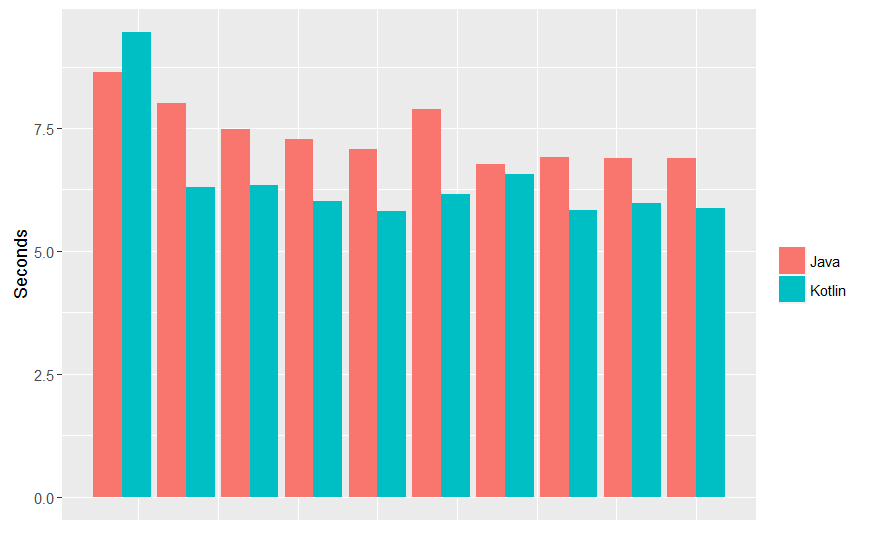
\includegraphics[scale=0.2]{kotlin}
	\\
	incremental builds with 1 core file changed
\end{center}

